\documentclass{standalone}

\usepackage[latin1]{inputenc}
\usepackage{tikz}

\usetikzlibrary{calc}

% GNUPLOT required
\begin{document}
\pagestyle{empty}

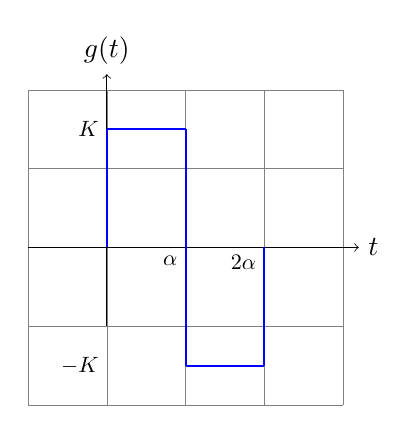
\begin{tikzpicture}[line width=0.25mm]
    \draw[very thin,color=gray] (-1,-2) grid (3,2);
    \draw[->, line width=0.1mm] (-1,0) -- (3.2,0) node[right] {$t$};
    \draw[->, line width=0.1mm] (0,-1) -- (0,2.2) node[above] {$g(t)$};

	% x(t)
    %\draw[color=blue, domain=-1:0] plot[id=x] function{x+1};
    %\draw[color=blue, domain=0:1] plot[id=x] function{-x+1};
    
	\draw[color=blue] (0,0) -- (0,1.5);
	\draw[color=blue] (0,1.5) -- (1,1.5);
	\draw[color=blue] (1,1.5) -- (1,-1.5);
	\draw[color=blue] (1,-1.5) -- (2,-1.5);
	\draw[color=blue] (2,-1.5) -- (2,0);
	
	%\draw[color=blue, domain=5:3.5] plot[id=x] function{0};% Para indicar la fucnción, se puede quitar los comentario y el último ;
        %node[above right] {$x(t)$};


	\draw ($(1,0) + (0,0)$) -- ($(1,0) + (0,0)$)
        node [below left,scale=0.8] {$\alpha$};
	\draw ($(2,0) + (0,0)$) -- ($(2,0) + (0,0)$)
        node [below left,scale=0.8] {$2\alpha$};
	\draw ($(0,1.5) + (0,0)$) -- ($(0,1.5) + (0,0)$)
        node [left,scale=0.8] {$K$};
	\draw ($(0,-1.5) + (0,0)$) -- ($(0,-1.5) + (0,0)$)
        node [left,scale=0.8] {$-K$};
	
\end{tikzpicture}


\end{document}
